In Exercises \ref{powergraphexfirst} - \ref{powergraphexlast}, use the given graphs along with Theorem \ref{linearrationalpowergraphs} to graph the given function.  Track at least two points and state the domain and range using interval notation.

\begin{center}

\begin{multicols}{2}

\begin{mfpic}[20]{-4}{4}{-1}{4}
\axes
\tlabel[cc](4, -0.5){\scriptsize $x$}
\tlabel[cc](0.5, 4){\scriptsize $y$}
\tlabel[cc](1.75,0.75){\scriptsize $(1,1)$}
\tlabel[cc](-1.75,0.75){\scriptsize $(-1,1)$}
\tlabel[cc](0.5,-0.5){\scriptsize $(0,0)$}
\penwd{1.25pt}
\arrow \reverse \arrow \parafcn{-1.5, 1.5,0.1}{(t**3,t**2)}
\point[4pt]{(-1,1), (0,0), (1,1)}
\tcaption{$f(x)=x^{\frac{2}{3}}$}
\end{mfpic}



\begin{mfpic}[20]{-4}{4}{-1}{4}
\axes
\tlabel[cc](4, -0.5){\scriptsize $t$}
\tlabel[cc](0.5, 4){\scriptsize $y$}
\tlabel[cc](2,1){\scriptsize $(1,1)$}
\tlabel[cc](0.5,-0.5){\scriptsize $(0,0)$}
\penwd{1.25pt}
\arrow  \function{0, 1.5,0.1}{x**3.14}
\point[4pt]{(0,0), (1,1)}
\tcaption{$g(t)=t^{\pi}$ \vphantom{{$f(x)=x^{\frac{2}{3}}$}}}
\end{mfpic}

\end{multicols}
\end{center}

\begin{multicols}{2}
\begin{enumerate}

\item $F(x) = (x-2)^{\frac{2}{3}}-1$ \label{powergraphexfirst}
\item $G(t) = (t+3)^{\pi} +1$

\setcounter{HW}{\value{enumi}}
\end{enumerate}
\end{multicols}

\begin{multicols}{2}
\begin{enumerate}
\setcounter{enumi}{\value{HW}}
\item $F(x) = 3-x^{\frac{2}{3}}$ 
\item $G(t) = (1-t)^{\pi}-2$  \vphantom{$F(x) = 3-x^{\frac{2}{3}}$ }

\setcounter{HW}{\value{enumi}}
\end{enumerate}
\end{multicols}


\begin{multicols}{2}
\begin{enumerate}
\setcounter{enumi}{\value{HW}}

\item $F(x) =(2x+5)^{\frac{2}{3}}+1$ \vphantom{$G(t) = \left( \dfrac{t+3}{2}\right)^{\pi}-1$}
\item $G(t) = \left( \dfrac{t+3}{2}\right)^{\pi}-1$ \label{powergraphexlast}
\setcounter{HW}{\value{enumi}}
\end{enumerate}
\end{multicols}

In Exercises \ref{findformulaforpowergraphfirst} - \ref{findformulaforpowergraphlast}, find a formula for each function below in the form $F(x) = a(bx-h)^{\frac{2}{3}}+k$.

\smallskip

\textbf{NOTE:}  There may be more than one solution!

\begin{multicols}{2}

\begin{enumerate}
\setcounter{enumi}{\value{HW}}

\item $~$ \label{findformulaforpowergraphfirst}  $y=F(x)$ %$F(x) = 2(x-1)^{\frac{2}{3}}-2$

\begin{mfpic}[20]{-4}{4}{-4}{4}
\axes
\tlabel[cc](4, -0.5){\scriptsize $x$}
\tlabel[cc](0.5, 4){\scriptsize $y$}
\tlabel[cc](1, -2.5){\scriptsize $(1,-2)$}
\tlabel[cc](2.5,-0.5){\scriptsize $(2,0)$}
\tlabel[cc](-0.5,-0.5){\scriptsize $(0,0)$}
\penwd{1.25pt}
\arrow \reverse \arrow \parafcn{-1.5, 1.5,0.1}{((t**3)+1,(2*(t**2))-2)}
\point[4pt]{(0,0), (1,-2), (2,0)}
\end{mfpic}
 



\item $~$ \label{findformulaforpowergraphlast} $y = F(x)$ %$F(x) =-(x+1)^{\frac{2}{3}} + 4$

\begin{mfpic}[10][20]{-10}{10}{-2}{6}
\axes
\tlabel[cc](10, -0.5){\scriptsize $x$}
\tlabel[cc](0.5, 6){\scriptsize $y$}
\tlabel[cc](-10, 0.5){\scriptsize $(-9,0)$}
\tlabel[cc](-1.5,4.5){\scriptsize $(-1,4)$}
\tlabel[cc](1.5,3){\scriptsize $(0,3)$}
\tlabel[cc](7,0.5){\scriptsize $(6,0)$}
\penwd{1.25pt}
\arrow \reverse \arrow \parafcn{-2.15,2.15 ,0.1}{((t**3)-1,4-(t**2))}
\point[4pt]{(-9,0), (7,0), (0,3), (-1,4)}
\end{mfpic}
 

\setcounter{HW}{\value{enumi}}

\end{enumerate}

\end{multicols}
\newpage

For each function in Exercises \ref{powerfcngraphexfirst} - \ref{powerfcngraphexlast} below 

\begin{itemize}

\item Analytically:

\begin{multicols}{3}

\begin{itemize}

\item find the domain.

\item find the axis intercepts.

\item analyze the end behavior.

\end{itemize}

\end{multicols}

\item Graph the function with help from a graphing utility and determine:

\begin{multicols}{2}

\begin{itemize}

\item  the range.

\item the local extrema, if they exist.

\end{itemize}

\end{multicols}

\begin{multicols}{2}

\begin{itemize}

\item intervals of increase/decrease.

\item any `unusual steepness' or `local' verticality.

\end{itemize}

\end{multicols}

\begin{multicols}{2}

\begin{itemize}

\item  vertical asymptotes.

\item  horizontal / slant asymptotes.

\end{itemize}

\end{multicols}

\item Construct a sign diagram for each function using the intercepts and graph.

\item  Comment on any observed symmetry.


\end{itemize}


\begin{multicols}{2}
\begin{enumerate}
\setcounter{enumi}{\value{HW}}

\item $f(x) = x^{\frac{2}{3}}(x - 7)^{\frac{1}{3}}$  \label{powerfcngraphexfirst}
\item $f(x) = x^{\frac{3}{2}}(x - 7)^{\frac{1}{3}}$ 


\setcounter{HW}{\value{enumi}}
\end{enumerate}
\end{multicols}

\begin{multicols}{2}
\begin{enumerate}
\setcounter{enumi}{\value{HW}}

\item $g(t) = 2t(t+3)^{-\frac{1}{3}}$ 
\item $g(t) = t^{\frac{3}{2}}(t-2)^{-\frac{1}{2}}$ 


\setcounter{HW}{\value{enumi}}
\end{enumerate}
\end{multicols}

\begin{multicols}{2}
\begin{enumerate}
\setcounter{enumi}{\value{HW}}

\item $f(x) = x^{0.4} (3-x)^{0.6}$ 
\item $f(x) = x^{0.5} (3-x)^{0.5}$ 


\setcounter{HW}{\value{enumi}}
\end{enumerate}
\end{multicols}

\begin{multicols}{2}
\begin{enumerate}
\setcounter{enumi}{\value{HW}}

\item $g(t) = 4t (9-t^2)^{-\sqrt{2}}$ 
\item $g(t) = 3(t^2+1)^{-\pi}$  \label{powerfcngraphexlast}


\setcounter{HW}{\value{enumi}}
\end{enumerate}
\end{multicols}

\begin{enumerate}
\setcounter{enumi}{\value{HW}}

\item \label{powerarcexercise}For each function $f(x)$ listed below, compute the average rate of change over the indicated interval.\footnote{See Definition \ref{arc} in Section \ref{AverageRateofChange} for a review of this concept, as needed.}  What trends do you observe?  How do your answers manifest themselves graphically?  Compare the results of this exercise with those of Exercise \ref{monomialarcexercise} in Section \ref{GraphsofPolynomials} and Exercise \ref{laurentarcexercise} in Section \ref{IntroRational}

\[ \begin{array}{|r||c|c|c|c|}  \hline

 f(x) &  [0.9, 1.1] & [0.99, 1.01] &[0.999, 1.001] & [0.9999, 1.0001]  \\ \hline
 x^{\frac{1}{2}} &&&&  \\  \hline
 x^{\frac{2}{3}} &&&&  \\ \hline
 x^{-0.23} &&&&   \\  \hline
 x^{\pi}  &&&&   \\  \hline

\end{array} \]

\item \label{WindChillTemperature} The \href{http://www.nws.noaa.gov/om/windchill/windchillglossary.shtml}{\underline{National Weather Service}} uses the following formula to calculate the wind chill: \[ W = 35.74 + 0.6215 \, T_{a} - 35.75\, V^{0.16} + 0.4275 \, T_{a} \, V^{0.16}  \] where $W$ is the wind chill temperature in $^{\circ}$F, $T_{a}$ is the air temperature in $^{\circ}$F, and  $V$ is the wind speed in miles per hour.  Note that $W$ is defined only for air temperatures at or lower than $50^{\circ}$F and wind speeds above $3$ miles per hour.

\begin{enumerate}

\item  Suppose the air temperature is $42^{\circ}$ and the wind speed is $7$ miles per hour. Find the wind chill temperature.  Round your answer to two decimal places.

\item  Suppose the air temperature is $37^{\circ}$F and the wind chill temperature is $30^{\circ}$F.  Find the wind speed.  Round your answer to two decimal places. 

\end{enumerate}

\item  As a follow-up to Exercise \ref{WindChillTemperature}, suppose the air temperature is $28^{\circ}$F.  

\begin{enumerate}

\item Use the formula from Exercise \ref{WindChillTemperature} to find an expression for the wind chill temperature as a function of the wind speed, $W(V)$.  

\item  \label{WindChill0} Solve $W(V) = 0$, round your answer to two decimal places,  and interpret.  

\item  Graph the function $W$ using a graphing utility and check your answer to part \ref{WindChill0}. 


\end{enumerate}


\item \label{pursuitfurther} Suppose Fritzy the Fox, positioned at a point $(x,y)$ in the first quadrant, spots Chewbacca the Bunny at $(0,0)$.   Chewbacca begins to run along a fence (the positive $y$-axis) towards his warren.  Fritzy, of course, takes chase and constantly adjusts his direction so that he is always running directly at Chewbacca.  If Chewbacca's speed is $v_{\mbox{\tiny$1$}}$ and  Fritzy's speed is $v_{\mbox{\tiny$2$}}$, the path Fritzy will take to intercept Chewbacca, provided $v_{\mbox{\tiny$2$}}$ is directly proportional to, but not equal to, $v_{\mbox{\tiny$1$}}$ is modeled by

\[ y = \dfrac{1}{2} \left(\dfrac{x^{1+ v_{1}/v_{2}}}{1+v_{\mbox{\tiny$1$}}/v_{\mbox{\tiny$2$}}}- \dfrac{x^{1-v_{\mbox{\tiny$1$}}/v_{\mbox{\tiny$2$}}}}{1-v_{\mbox{\tiny$1$}}/v_{\mbox{\tiny$2$}}}\right) + \dfrac{v_{\mbox{\tiny$1$}} v_{\mbox{\tiny$2$}}}{v_{\mbox{\tiny$2$}}^2-v_{\mbox{\tiny$1$}}^2} \]

\begin{enumerate}

\item  Determine the path that Fritzy will take if he runs exactly twice as fast as Chewbacca;  that is, $v_{\mbox{\tiny$2$}} = 2v_{\mbox{\tiny$1$}}$. Use your calculator to graph this path for $x \geq 0$.  What is the significance of the $y$-intercept of the graph?

\item  Determine the path Fritzy will take if Chewbacca runs exactly twice as fast as he does;  that is, $v_{\mbox{\tiny$1$}} = 2v_{\mbox{\tiny$2$}}$.  Use a graphing utility to graph this path for $x > 0$.  Describe the behavior of $y$ as $x \rightarrow 0^{+}$ and interpret this physically.

\item  With the help of your classmates, generalize parts (a) and (b) to two cases:  $v_{\mbox{\tiny$2$}} > v_{\mbox{\tiny$1$}}$ and $v_{\mbox{\tiny$2$}} < v_{\mbox{\tiny$1$}}$.   We will discuss the case of $v_{\mbox{\tiny$1$}} = v_{\mbox{\tiny$2$}}$ in Exercise \ref{pursuitlog} in Section \ref{ExpLogApplications}.

\end{enumerate}

\setcounter{HW}{\value{enumi}}
\end{enumerate}

\newpage

\subsection{Answers}

\begin{multicols}{2}
\begin{enumerate}

\item  $F(x) = (x-2)^{\frac{2}{3}}-1$ \\

\begin{mfpic}[20]{-2}{6}{-2}{3}
\axes
\tlabel[cc](6, -0.5){\scriptsize $x$}
\tlabel[cc](0.25, 3){\scriptsize $y$}
\tlabel[cc](3.5,-0.5){\scriptsize $(3,0)$}
\tlabel[cc](0.5,-0.5){\scriptsize $(1,0)$}
\tlabel[cc](2,-1.5){\scriptsize $(2,-1)$}
\penwd{1.25pt}
\arrow \reverse \arrow \parafcn{-1.5, 1.5,0.1}{(t**3+2,t**2-1)}
\point[4pt]{(1,0), (2,-1), (3,0)}
\tcaption{Domain:  $(-\infty, \infty)$, Range:  $[-1, \infty)$}
\end{mfpic}


\columnbreak


\item $G(t) = (t+3)^{\pi} +1$ \vphantom{$F(x) = (x-2)^{\frac{2}{3}}-1$}\\

\begin{mfpic}[20]{-7}{1}{0}{5}
\axes
\tlabel[cc](1, -0.5){\scriptsize $t$}
\tlabel[cc](0.5, 5){\scriptsize $y$}
\tlabel[cc](-1,2){\scriptsize $(-2,2)$}
\tlabel[cc](-2.5,0.5){\scriptsize $(-3,1)$}
\penwd{1.25pt}
\arrow  \function{-3,-1.5,0.1}{((x+3)**3.14)+1}
\point[4pt]{(-3,1), (-2,2)}
\tcaption{Domain:  $[-3, \infty)$, Range:  $[1, \infty)$}
\end{mfpic}


\setcounter{HW}{\value{enumi}}
\end{enumerate}
\end{multicols}

\begin{multicols}{2}
\begin{enumerate}
\setcounter{enumi}{\value{HW}}
\item  $F(x) = 3-x^{\frac{2}{3}} = (-1)x^{\frac{2}{3}} + 3$  \\

\begin{mfpic}[20]{-4}{4}{-1}{4}
\axes
\tlabel[cc](4, -0.5){\scriptsize $x$}
\tlabel[cc](0.5, 4){\scriptsize $y$}
\tlabel[cc](1.5,2.25){\scriptsize $(1,2)$}
\tlabel[cc](-1.75,2.25){\scriptsize $(-1,2)$}
\tlabel[cc](0.75,3){\scriptsize $(0,3)$}
\penwd{1.25pt}
\arrow \reverse \arrow \parafcn{-1.5, 1.5,0.1}{(t**3,3-(t**2))}
\point[4pt]{(-1,2), (0,3), (1,2)}
\tcaption{Domain: $(-\infty, \infty)$, Range: $(-\infty,3]$} 
\end{mfpic}


\columnbreak


\item  $G(t) = (1-t)^{\pi}-2 = ((-1)t+1)^{\pi}-2$  \vphantom{$F(x) = 3-x^{\frac{2}{3}}$} \\

\begin{mfpic}[20]{-4}{4}{-3}{2}
\axes
\tlabel[cc](4, -0.5){\scriptsize $t$}
\tlabel[cc](0.5, 2){\scriptsize $y$}
\tlabel[cc](2,-2){\scriptsize $(1,-2)$}
\tlabel[cc](0.75,-1){\scriptsize $(0,-1)$}
\penwd{1.25pt}
\arrow  \reverse \function{-0.5, 1,0.1}{((1-x)**3.14)-2}
\point[4pt]{(0,-1), (1,-2)}
\tcaption{Domain:  $(-\infty, 1]$, Range: $[-2, \infty)$}
\end{mfpic}

\setcounter{HW}{\value{enumi}}
\end{enumerate}
\end{multicols}

\begin{multicols}{2}
\begin{enumerate}
\setcounter{enumi}{\value{HW}}
\item  $F(x) =(2x+5)^{\frac{2}{3}}+1$ \vphantom{$G(t) = \left( \dfrac{t+3}{2}\right)^{\pi}-1$}  \\

\begin{mfpic}[20]{-6.5}{1.5}{-1}{4}
\axes
\tlabel[cc](1.5, -0.5){\scriptsize $x$}
\tlabel[cc](0.5, 4){\scriptsize $y$}
\tlabel[cc](-4,1.75){\scriptsize $(-3,2)$}
\tlabel[cc](-2.5,0.5){\scriptsize $\left(-\frac{5}{2},1 \right)$}
\tlabel[cc](-1,1.75){\scriptsize $(-2,2)$}
\penwd{1.25pt}
\arrow \reverse \arrow \parafcn{-1.6, 1.6,0.1}{( 0.5*( (t**3)-5),(t**2)+1)}
\point[4pt]{(-3,2), (-2.5,1), (-2,2)}
\tcaption{Domain: $(-\infty, \infty)$, Range: $[1, \infty)$}
\end{mfpic}


\columnbreak


\item  $G(t) = \left( \dfrac{t+3}{2}\right)^{\pi}-1= \left( \frac{1}{2} \, t + \frac{3}{2}\right)^{\pi} -1$\\

\begin{mfpic}[20]{-4}{4}{-2}{3}
\axes
\tlabel[cc](4, -0.5){\scriptsize $t$}
\tlabel[cc](0.5, 3){\scriptsize $y$}
\tlabel[cc](-3,-1.5){\scriptsize $(-3,-1)$}
\tlabel[cc](-1.5,0.5){\scriptsize $(-1,0)$}
\penwd{1.25pt}
\arrow  \function{-3, -0.2,0.1}{(((x+3)/2)**3.14)-1}
\point[4pt]{(-3,-1), (-1,0)}
\tcaption{Domain:  $[-3, \infty)$, Range: $[-1, \infty)$}
\end{mfpic}

\setcounter{HW}{\value{enumi}}
\end{enumerate}
\end{multicols}

\begin{multicols}{2}

\begin{enumerate}
\setcounter{enumi}{\value{HW}}

\item One solution is: $F(x) = 2(x-1)^{\frac{2}{3}}-2$

\item  One solution is: $F(x) =-(x+1)^{\frac{2}{3}} + 4$


\setcounter{HW}{\value{enumi}}
\end{enumerate}

\end{multicols}

\newpage

\begin{enumerate}
\setcounter{enumi}{\value{HW}}

\item \begin{multicols}{2} 
$f(x) = x^{\frac{2}{3}}(x - 7)^{\frac{1}{3}}$\\
Domain: $(-\infty, \infty)$\\
Intercepts: $(0,0)$, $(7,0)$\\
Graph: \\

\begin{mfpic}[10]{-4}{10}{-5}{5.5}
\axes
\tlabel[cc](10,-0.5){\scriptsize $x$}
\tlabel[cc](0.5,5.5){\scriptsize $y$}
\tlabel[cc](5,-5){\scriptsize $\approx (4.667, -3.704)$}
\xmarks{-3 step 1 until 9}
\ymarks{-4 step 1 until 5}
\tlpointsep{4pt}
\tiny
\axislabels {x}{{$-3 \hspace{6pt}$} -3, {$-2 \hspace{6pt}$} -2, {$-1 \hspace{6pt}$} -1, {$1$} 1, {$2$} 2, {$3$} 3, {$4$} 4, {$5$} 5, {$6$} 6,  {$8$} 8, {$9$} 9}
\axislabels {y}{{$-4$} -4, {$-3$} -3, {$-2$} -2,  {$1$} 1, {$2$} 2, {$3$} 3, {$4$} 4, {$5$} 5}
\normalsize
\point[4pt]{(0,0), (7,0), (4.667, -3.704)}
\dashed \polyline{(-3, -5.33), (9, 6.67)}
\penwd{1.25pt}
\arrow \reverse \function{-3,0,0.1}{-((x**2)**(1/3))*((7 - x)**(1/3))}
\function{0,7,0.1}{-((x**2)**(1/3))*((7 - x)**(1/3))}
\arrow \function{7,9,0.1}{((x**2)**(1/3))*((x - 7)**(1/3))}
\end{mfpic}

\vfill
\columnbreak

$\ds{\lim_{x \rightarrow - \infty} f(x) = - \infty}$, $\ds{\lim_{x \rightarrow \infty} f(x) = \infty}$\footnote{Using Calculus it can be shown that $y = x - \frac{7}{3}$ is a slant asymptote of this graph.}\\
Range: $(-\infty, \infty)$\\
Local minimum: $\approx (4.667, -3.704)$\\
Local maximum: $(0,0)$ (this is a cusp) \\
Increasing: $(-\infty, 0]$, $\approx [4.667, \infty)$\\
Decreasing: $[0, 4.667]$\\
Unusual steepness at $x = 7$\\

Sign Diagram:\\

\smallskip

\begin{mfpic}[10]{-3}{10}{-2}{2}
\arrow \reverse \arrow \polyline{(-3,0),(10,0)}
\xmarks{0,7}
\tlabel[cc](-1.5,1){$(-)$}
\tlabel[cc](0,-1){$0$}
\tlabel[cc](0,1){$0$}
\tlabel[cc](3.5,1){$(-)$}
\tlabel[cc](7,-1){$7$}
\tlabel[cc](7,1){$0$}
\tlabel[cc](8.5,1){$(+)$}
\end{mfpic}



\end{multicols}

\item \begin{multicols}{2} 
$f(x) = x^{\frac{3}{2}}(x - 7)^{\frac{1}{3}}$\\
Graph: \\
\begin{mfpic}[15][3]{-1}{8.5}{-20}{30}
\axes
\tlabel[cc](8.5,-3){\scriptsize $x$}
\tlabel[cc](0.5,30){\scriptsize $y$}
\tlabel[cc](6,-18){\scriptsize $\approx (5.727, -14.854)$}
\xmarks{1 step 1 until 8}
\ymarks{-15 step 5 until 25}
\tlpointsep{4pt}
\scriptsize
\axislabels {x}{ {$2$} 2, {$3$} 3, {$4$} 4, {$5$} 5, {$6$} 6,  {$8$} 8}
\axislabels {y}{{$-15$} -15, {$-10$} -10, {$-5$} -5, {$5$} 5, {$10$} 10, {$15$} 15, {$20$} 20, {$25$} 25}
\normalsize
\point[4pt]{(0,0), (7,0), (5.727, -14.854)}
\penwd{1.25pt}
\function{0,7,0.1}{-(x**1.5)*((7 - x)**(1/3))}
\arrow \function{7,8.5,0.1}{(x**1.5)*((x - 7)**(1/3))}
\end{mfpic}


\vfill
\columnbreak

Domain: $[0, \infty)$\\
Intercepts: $(0,0)$, $(7,0)$\\
$\ds{\lim_{x \rightarrow \infty} f(x) = \infty}$\\
Range:  $\approx [-14.854, \infty)$\\
Local minimum:  $\approx (5.727, -14.854)$\\
Increasing: $\approx [5.727, \infty)$\\
Decreasing: $\approx [0, 5.727]$\\
Unusual steepness at $x = 7$\\
Sign Diagram:\\

\smallskip

\begin{mfpic}[15]{0}{10}{-1}{1}
\reverse \arrow \polyline{(0,0),(10,0)}
\xmarks{0, 7}
\tlabel[cc](0,-0.5){$0$}
\tlabel[cc](0,0.5){$0$}
\tlabel[cc](3.5, 0.5){$(-)$}
\tlabel[cc](7,-0.5){$7$}
\tlabel[cc](7,0.5){$0$}
\tlabel[cc](8, 0.5){$(+)$}
\end{mfpic}


\end{multicols}

\setcounter{HW}{\value{enumi}}
\end{enumerate}


\begin{enumerate}
\setcounter{enumi}{\value{HW}}

\item \begin{multicols}{2} 
 $g(t) = 2t(t+3)^{-\frac{1}{3}}$ \\
Graph: \\

\begin{mfpic}[10][5]{-10}{5}{-10}{10}
\axes
\tlabel[cc](5,-0.5){\scriptsize $t$}
\tlabel[cc](0.5,10){\scriptsize $y$}
\tlabel[cc](-6,5){\scriptsize $\approx (-4.5, 7.862)$}
\xmarks{-9 step 1 until 4}
\ymarks{-8 step 2 until 8}
\tlpointsep{4pt}
\tiny
\axislabels {x}{{$-9 \hspace{6pt}$} -9, {$-8 \hspace{6pt}$} -8, {$-7 \hspace{6pt}$} -7, {$-6 \hspace{6pt}$} -6, {$-5 \hspace{6pt}$} -5, {$-4 \hspace{6pt}$} -4, {$-3 \hspace{6pt}$} -3, {$-2 \hspace{6pt}$} -2, {$-1 \hspace{6pt}$} -1, {$1$} 1, {$2$} 2, {$3$} 3, {$4$} 4}
\axislabels {y}{ {$-8$} -8,  {$-6$} -6, {$-4$} -4, {$-2$} -2,   {$2$} 2, {$4$} 4,  {$6$} 6,  {$8$} 8}
\normalsize
\dashed \polyline{(-3,-9), (-3, 10)}
\point[4pt]{(0,0), (-4.5, 7.862)}
\penwd{1.25pt}
\arrow \reverse \arrow \function{-9,-3.2,0.1}{-(2*x)/((-x-3)**(1/3))}
\arrow \reverse \function{-2.8,0,0.1}{(2*x)/((x+3)**(1/3))}
\arrow \function{0,5,0.1}{(2*x)/((x+3)**(1/3))}

\end{mfpic}

\vfill
\columnbreak

Domain: $(-\infty, -3) \cup (-3, \infty)$\\
Intercept: $(0,0)$\\
$\ds{\lim_{t \rightarrow -\infty} g(t) = \infty}$\\
$\ds{\lim_{t \rightarrow \infty} g(t) = \infty}$\\
Range: $(-\infty, \infty)$\\
Local minimum: $\approx (-4.5, 7.862)$\\
Increasing: $\approx [-4.5, -3)$, $(-3,\infty)$ \\
Decreasing: $\approx (-\infty, -4.5]$\\
Vertical Asymptote:  $t = -3$\\
Sign Diagram:\\

\smallskip

\begin{mfpic}[10]{-3}{10}{-2}{2}
\arrow \reverse \arrow \polyline{(-3,0),(10,0)}
\xmarks{0,7}
\tlabel[cc](-1.5,1){$(+)$}
\tlabel[cc](0,-1){$-3 \hspace{6pt}$}
\tlabel[cc](0,1){\textinterrobang}
\tlabel[cc](3.5,1){$(-)$}
\tlabel[cc](7,-1){$0$}
\tlabel[cc](7,1){$0$}
\tlabel[cc](8.5,1){$(+)$}
\end{mfpic}



\end{multicols}

\item \begin{multicols}{2} 
$g(t)= t^{\frac{3}{2}}(t-2)^{-\frac{1}{2}}$\\
Domain:  $(2, \infty)$\\
$\ds{\lim_{t \rightarrow \infty} g(t) = \infty}$\\
Graph: \\
\begin{mfpic}[15][10]{-1}{10}{-1}{10}
\axes
\tlabel[cc](10,-0.5){\scriptsize $t$}
\tlabel[cc](0.5,10){\scriptsize $y$}
\xmarks{1 step 1 until 9}
\ymarks{1 step 2 until 9}
\tlpointsep{4pt}
\tiny
\axislabels {x}{{$1$} 1, {$2$} 2, {$3$} 3, {$4$} 4, {$5$} 5, {$6$} 6,  {$7$} 7, {$8$} 8, {$9$} 9}
\axislabels {y}{{$1$} 1,  {$3$} 3, {$5$} 5,  {$7$} 7,  {$9$} 9}
\normalsize
\dashed \polyline{(2,5), (2,9)}
\dashed \polyline{(4,5), (9,10)}
\gclear \tlabelrect(3,4){\scriptsize $\approx (3, 5.196)$}
\point[4pt]{(3, 5.196)}
\penwd{1.25pt}
\arrow \reverse \arrow \function{2.1,8.75,0.1}{(x**1.5)*((x - 2)**(-0.5))}
\end{mfpic}


\vfill
\columnbreak
$\ds{\lim_{t \rightarrow \infty} g(t) = \infty}$\footnote{Using Calculus it can be shown that $y = t+1$ is a slant asymptote of this graph.}\\
Range:  $\approx [5.196, \infty)$\\
Local minimum:  $\approx (3, 5.196)$\\
Increasing: $\approx [3, \infty)$\\
Decreasing: $\approx (2,3]$\\
Vertical asymptote:  $t = 2$\\
Sign Diagram:\\

\smallskip

\begin{mfpic}[15]{0}{10}{-1}{1}
\reverse \arrow \polyline{(0,0),(4,0)}
\xmarks{0}
\tlabel[cc](0,-0.5){$2$}
\tlabel[cc](0,0.5){\textinterrobang}
\tlabel[cc](2, 0.5){$(+)$}
\end{mfpic}


\end{multicols}

\setcounter{HW}{\value{enumi}}
\end{enumerate}



\begin{enumerate}
\setcounter{enumi}{\value{HW}}

\item \begin{multicols}{2} 
 $f(x) = x^{0.4}(3-x)^{0.6}$ \\
Graph: \\
\begin{mfpic}[20]{-2}{5}{-2}{4}
\axes
\tlabel[cc](5,-0.5){\scriptsize $x$}
\tlabel[cc](0.5,4){\scriptsize $y$}
\tlabel[cc](2,2){\scriptsize $\approx (1.2, 1.531)$}
\xmarks{-1 step 1 until 4}
\ymarks{-1 step 1 until 3}
\tlpointsep{4pt}
\tiny
\axislabels {x}{ {$-1 \hspace{6pt}$} -1, {$1$} 1, {$2$} 2,  {$4$} 4}
\axislabels {y}{{$-1$} -1,   {$2$} 2,   {$3$} 3,   {$4$} 4}
\normalsize
%\dashed \polyline{(-3,-9), (-3, 10)}
\point[4pt]{(0,0), (3,0), (1.2, 1.531)}
\penwd{1.25pt}
\function{0,3,0.1}{(x**0.4)*((3-x)**0.6)}

\end{mfpic}

\vfill
\columnbreak


Domain: $[0,3]$\\
Intercepts: $(0,0)$, $(3,0)$\\
Range: $\approx [0, 1.5]$\\
Increasing: $\approx [0, 1.2]$ \\
Decreasing: $\approx [1.2, 3]$\\
Unusual Steepness:\footnote{Note you may need to zoom in to see this.}  $x=0$, $x = 3$\\
Sign Diagram:\\

\smallskip

\begin{mfpic}[10]{-3}{10}{-2}{2}
 \polyline{(0,0),(7,0)}
\xmarks{0,7}
\tlabel[cc](0,-1){$0$}
\tlabel[cc](0,1){$0$}
\tlabel[cc](3.5,1){$(+)$}
\tlabel[cc](7,-1){$3$}
\tlabel[cc](7,1){$0$}
\end{mfpic}




\end{multicols}

\item \begin{multicols}{2} 
 $f(x) = x^{0.5}(3-x)^{0.5}$ \\
Graph: \\
\begin{mfpic}[20]{-2}{5}{-2}{4}
\axes
\tlabel[cc](5,-0.5){\scriptsize $x$}
\tlabel[cc](0.5,4){\scriptsize $y$}
\tlabel[cc](2,2){\scriptsize $\approx (1.5, 1.5)$}
\xmarks{-1 step 1 until 4}
\ymarks{-1 step 1 until 3}
\tlpointsep{4pt}
\tiny
\axislabels {x}{ {$-1 \hspace{6pt}$} -1, {$1$} 1, {$2$} 2,  {$4$} 4}
\axislabels {y}{{$-1$} -1,   {$1$} 1,  {$2$} 2,   {$3$} 3}
\normalsize
\point[4pt]{(0,0), (3,0), (1.5, 1.5)}
\penwd{1.25pt}
\function{0,3,0.1}{(x**0.5)*((3-x)**0.5)}
\end{mfpic}

\vfill
\columnbreak

Domain: $[0,3]$\\
Intercepts: $(0,0)$, $(3,0)$\\
Range: $\approx [0, 1.5]$\\
Increasing: $\approx [0, 1.5]$ \\
Decreasing: $\approx [1.5, 3]$\\
Unusual Steepness:\footnote{Note you may need to zoom in to see this.}  $x=0$, $x = 3$\\
Sign Diagram:\\

\smallskip

\begin{mfpic}[10]{-3}{10}{-2}{2}
 \polyline{(0,0),(7,0)}
\xmarks{0,7}
\tlabel[cc](0,-1){$0$}
\tlabel[cc](0,1){$0$}
\tlabel[cc](3.5,1){$(+)$}
\tlabel[cc](7,-1){$3$}
\tlabel[cc](7,1){$0$}
\end{mfpic}
\end{multicols}
\setcounter{HW}{\value{enumi}}
\end{enumerate}

\newpage

\begin{enumerate}
\setcounter{enumi}{\value{HW}}

\item \begin{multicols}{2} 
$g(t) = 4t (9-t^2)^{-\sqrt{2}}$\\
Graph: \\
\begin{mfpic}[15]{-4}{4}{-3}{3}
\axes
\tlabel[cc](4,-0.5){\scriptsize $t$}
\tlabel[cc](0.5,4){\scriptsize $y$}
\xmarks{-2 step 1 until 2}
\ymarks{-2 step 1 until 2}
\tlpointsep{4pt}
\tiny
\axislabels {x}{ {$-2 \hspace{6pt}$} -2,{$-1 \hspace{6pt}$} -1, {$1$} 1, {$2$} 2}
\axislabels {y}{{$-2$} -2, {$-1$} -1,   {$1$} 1,   {$2$} 2}
\normalsize
\dashed \polyline{(-3,-3), (-3, 3)}
\dashed \polyline{(3,-3), (3, 3)}
\point[4pt]{(0,0)}
\penwd{1.25pt}
\arrow \reverse \arrow  \function{-2.6,2.6,0.1}{4*x/((9-(x**2))**1.414)}
\end{mfpic}

\vfill
\columnbreak
 Domain: $(-3, 3)$\\
Intercepts: $(0,0)$\\
Range: $(-\infty, \infty)$\\
$\ds{\lim_{t \rightarrow -3^{+}} g(t) = -\infty}$, $\ds{\lim_{t \rightarrow 3^{-}} g(t) = \infty}$ \\
Vertical asymptotes:  $t = -3$ and $t = 3$\\
Increasing: $(-3,3)$ \\
Sign Diagram:\\

\smallskip

\begin{mfpic}[10]{-5}{5}{-2}{2}
\polyline{(-5,0),(5,0)}
\xmarks{-5,0,5}
\tlabel[cc](-5,-1){$-3 \hspace{6pt}$}
\tlabel[cc](-5,1){\textinterrobang}
\tlabel[cc](-2.5,1){$(-)$}
\tlabel[cc](0,-1){$0$}
\tlabel[cc](0,1){$0$}
\tlabel[cc](2.5,1){$(+)$}
\tlabel[cc](5,-1){$3$}
\tlabel[cc](5,1){\textinterrobang}
\end{mfpic}

Note:  $g$ is odd

\end{multicols}

\item \begin{multicols}{2} 
$g(t) = 3(t^2+1)^{-\pi}$ \\
Domain: $(-\infty, \infty)$\\
Graph: \\
\begin{mfpic}[20]{-4}{4}{-1}{4}
\axes
\tlabel[cc](4,-0.5){\scriptsize $t$}
\tlabel[cc](0.5,4){\scriptsize $y$}
\xmarks{-3 step 1 until 3}
\ymarks{1 step 1 until 3}
\tlpointsep{4pt}
\tiny
\axislabels {x}{ {$-3 \hspace{6pt}$} -3,{$-2 \hspace{6pt}$} -2,{$-1 \hspace{6pt}$} -1, {$1$} 1, {$2$} 2, {$3$} 3}
\axislabels {y}{ {$1$} 1,   {$2$} 2,   {$3$} 3}
\normalsize
\point[4pt]{(0,3)}
\penwd{1.25pt}
\arrow \reverse \arrow  \function{-3,3,0.1}{3/(((x**2)+1)**3.14)}
\end{mfpic}

\vfill
\columnbreak

Intercept: $(0,3)$\\
$\ds{\lim_{t \rightarrow -\infty} g(t) =0}$ \\
$\ds{\lim_{t \rightarrow \infty} g(t) =0}$ \\
Range: $(0, 3]$\\
Increasing: $(-\infty, 0]$ \\
Decreasing: $[0, \infty)$\\
Horizontal asymptote:  $y =0$\\
Sign Diagram:\\

\vspace*{-0.2in}

\begin{mfpic}[10]{-5}{5}{-2}{2}
 \arrow \reverse \arrow \polyline{(-5,0),(5,0)}

\tlabel[cc](0,1){$(+)$}

\end{mfpic}

Note:  $g$ is even

\end{multicols}
\setcounter{HW}{\value{enumi}}
\end{enumerate}

\begin{enumerate}
\setcounter{enumi}{\value{HW}}

\item As in  Exercise \ref{monomialarcexercise} in Section \ref{GraphsofPolynomials} and Exercise \ref{laurentarcexercise} in Section \ref{IntroRational}, the slopes of these curves near $x = 1$ approach the value of the exponent on $x$.

\[ \begin{array}{|r||c|c|c|c|}  \hline

 f(x) &  [0.9, 1.1] & [0.99, 1.01] &[0.999, 1.001] & [0.9999, 1.0001]  \\ \hline
 x^{\frac{1}{2}} & 0.5006 & \approx \frac{1}{2} & \approx \frac{1}{2} & \approx \frac{1}{2} \\ [5pt] \hline
 x^{\frac{2}{3}} & 0.6672 & 0.6667 & \approx \frac{2}{3} & \approx \frac{2}{3}  \\ [5pt] \hline
 x^{-0.23} & -0.2310 & \approx -0.23 &\approx -0.23 &  \approx -0.23  \\  \hline
 x^{\pi}  &3.1544 & 3.1417 & \approx \pi & \approx \pi   \\  \hline

\end{array} \]

\item

\begin{enumerate}

\item  $W \approx 37.55^{\circ}$F.

\item  $V \approx 9.84$ miles per hour.

\end{enumerate}

\item 

\begin{enumerate}

\item $W(V) = 53.142 - 23.78 V^{0.16}$.  Since we are told in Exercise \ref{WindChillTemperature} that wind chill is only effect for wind speeds of more than 3 miles per hour, we restrict the domain to $V > 3$.

\item $W(V)=0$ when $V \approx 152.29$.  This means, according to the model, for the wind chill temperature to be $0^{\circ}$F, the wind speed needs to be $152.29$ miles per hour.

\newpage

\item The graph of $y = W(V)$ is below.  \\

\centerline{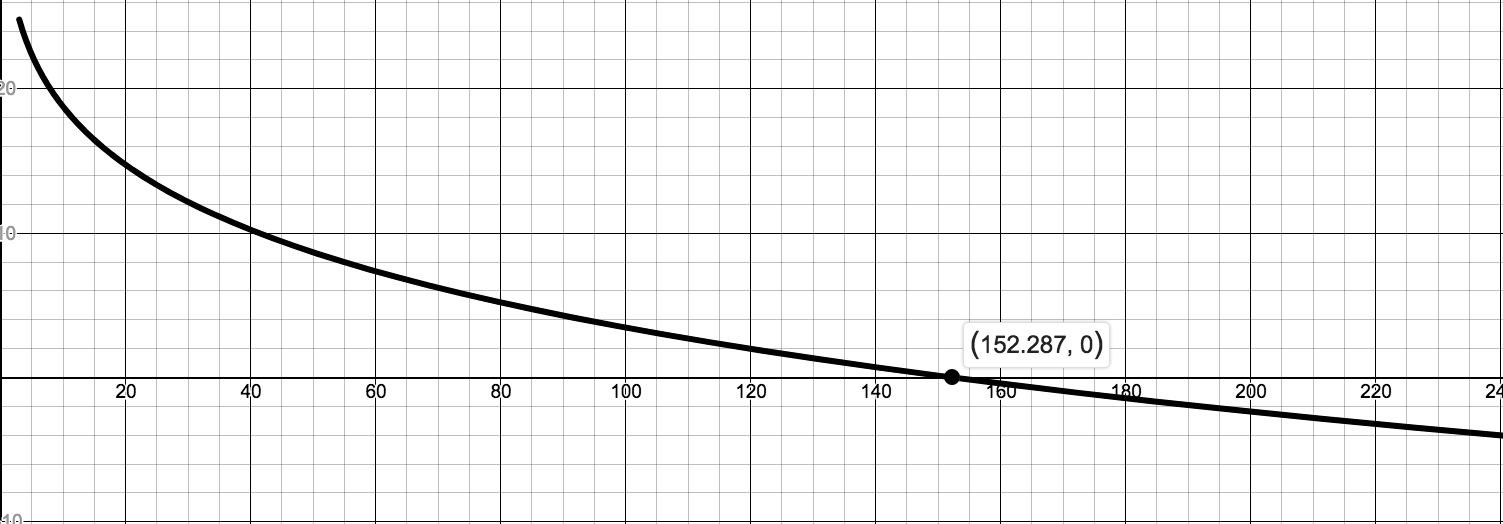
\includegraphics[height=1.75in]{./PowerFunctionsGraphics/WINDCHILL.jpg}}

\end{enumerate}



\item \begin{enumerate}

\item  $y = \frac{1}{3}x^{\frac{3}{2}} - x^{\frac{1}{2}} + \frac{2}{3}$.  The point $\left(0,\frac{2}{3}\right)$ is when Fritzy's path crosses Chewbacca's path - in other words, where Fritzy catches Chewbacca.

\begin{center} 

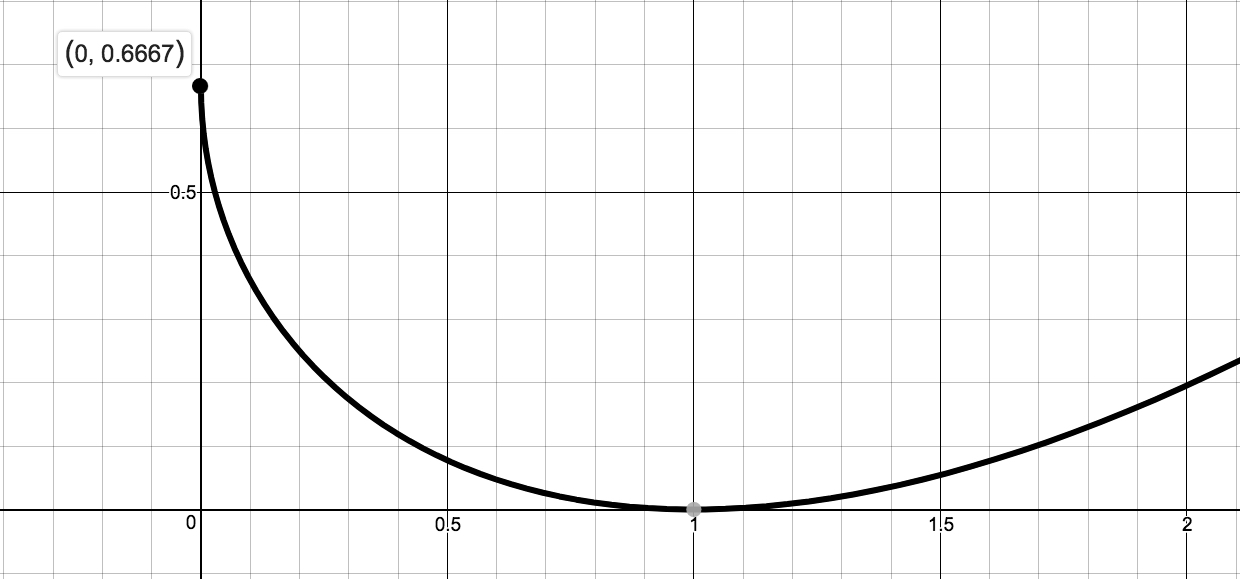
\includegraphics[height=2in]{./PowerFunctionsGraphics/PURSUIT01.jpg}

 $y = \frac{1}{3}x^{\frac{3}{2}} - x^{\frac{1}{2}} + \frac{2}{3}$

\end{center}

\item $y = \frac{1}{6}x^3+\frac{1}{2}x^{-1} - \frac{2}{3}$.  We find as $x \rightarrow 0^{+}$, $y \rightarrow \infty$ which means, in this case, Fritzy's pursuit never ends;  he never catches Chewbacca. This makes sense since Chewbacca has a head start and is running faster than Fritzy.

\begin{center} 

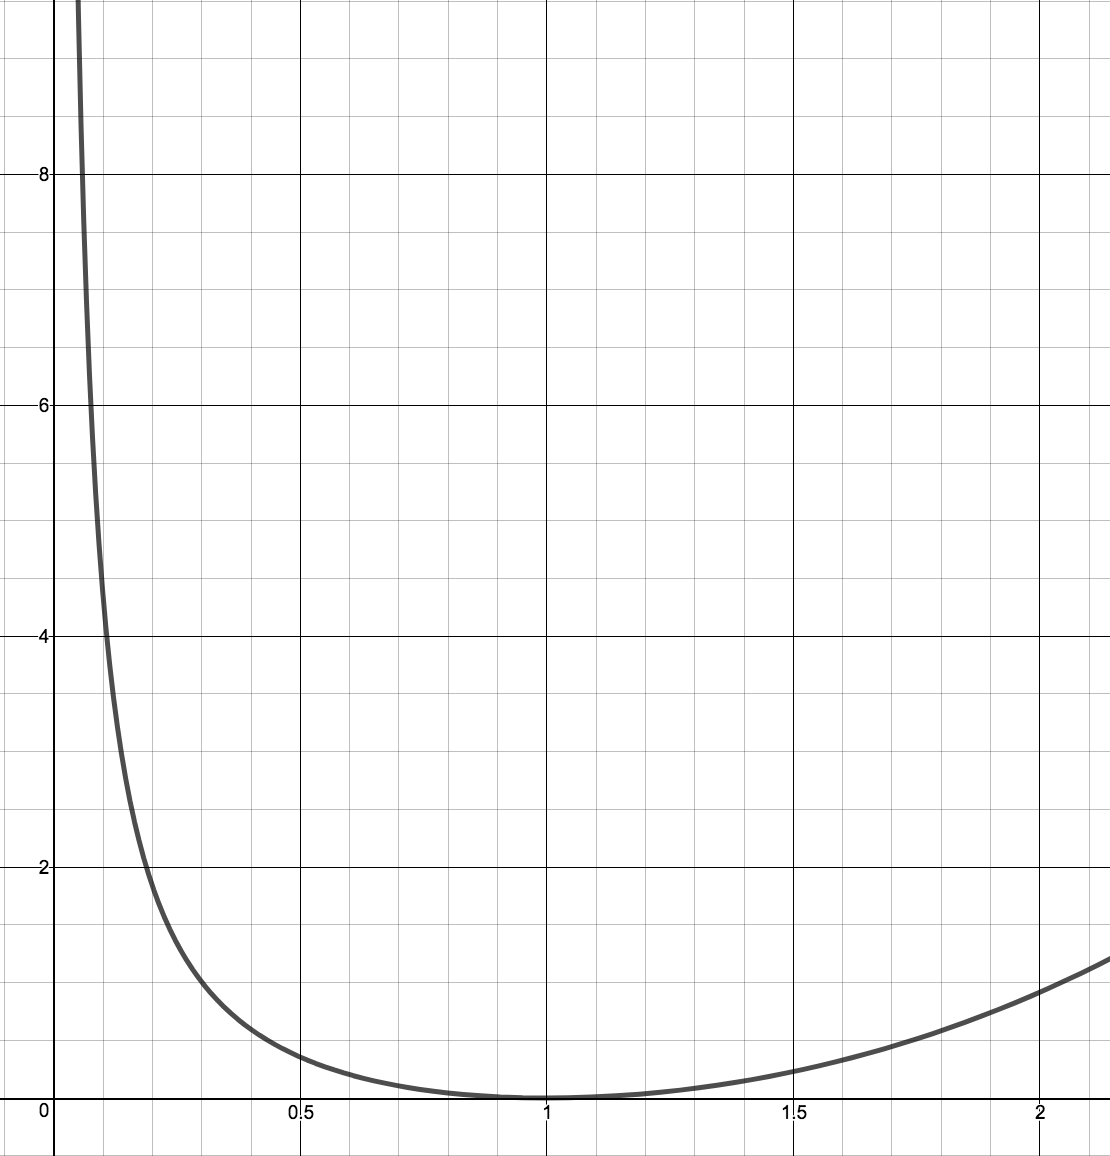
\includegraphics[height=2in]{./PowerFunctionsGraphics/PURSUIT02.jpg}

 $y = \frac{1}{6}x^3+\frac{1}{2}x^{-1} - \frac{2}{3}$

\end{center}


\end{enumerate}






\setcounter{HW}{\value{enumi}}
\end{enumerate}


